\documentclass[11pt]{article}
\usepackage{amsmath,amsfonts,amssymb,amsthm}
\usepackage{times}

\usepackage{geometry}
\geometry{verbose,tmargin=2cm,bmargin=2.5cm,lmargin=2.5cm,rmargin=2.5cm}

\usepackage{graphicx}
\graphicspath{ {./images/} }
\usepackage[ruled,vlined]{algorithm2e}

\makeatletter

\newtheorem{theorem}{Theorem}[section]
\newtheorem{lemma}[theorem]{Lemma}
\newtheorem{corollary}[theorem]{Corollary}
\newtheorem{claim}[theorem]{Claim}

\theoremstyle{definition}
\newtheorem{definition}[theorem]{Definition}
\theoremstyle{definition}
\newtheorem{example}[theorem]{Example}

\makeatother


%%% fill in details here
\def \lecturenum  {3}
\def \lecturedate {April 6, 2020}
\def \scribe      {Ilya Osadchiy}
%%%

\newcommand{\todo}[1]{\textbf{\textcolor{red}{TODO: #1}}}

%\def\pinv{\dag}

\DeclareMathOperator*{\argmin}{\arg\min}
\DeclareMathOperator*{\argmax}{\arg\max}


\def\X{{\mathcal X}}
\def\H{{\mathcal H}}
\def\Y{{\mathcal Y}}
\def\D{{\mathcal D}}
\def\L{{\mathcal L}}
\def\F{{\mathcal F}}
\def\mP{{\mathcal P}}
\def\reals{{\mathbb R}}
\def\R{{\mathcal R}}
\def\fhat{{\ensuremath{\hat{f}}}}
\def\mH{\mathcal{H}}
\newcommand{\at}{\makeatletter @\makeatother}

\DeclareMathOperator{\clip}{clip}
\def\norm#1{\mathopen\| #1 \mathclose\|}% use instead of $\|x\|$

\newcommand{\proj}{\mathop{\Pi}}

\newcommand{\err}{\mathop{\mbox{\rm error}}}
\newcommand{\rank}{\mathop{\mbox{\rm rank}}}
\newcommand{\ellipsoid}{{\mathcal E}}
\newcommand{\sround}{\mathop{\mbox{\rm SmartRound}}}
\newcommand{\round}{\mathop{\mbox{\rm round}}}
\newcommand{\myspan}{\mathop{\mbox{\rm span}}}
\newcommand{\edges}{\mathop{\mbox{\rm edges}}}
\newcommand{\conv}{\mathop{\mbox{\rm conv}}}
\newcommand{\sign}{\mathop{\mbox{\rm sign}}}
\newcommand{\poly}{\mathop{\mbox{\rm poly}}}

\newcommand{\ignore}[1]{}
\newcommand{\equaldef}{\stackrel{\text{\tiny def}}{=}}
\newcommand{\equaltri}{\triangleq}
\newcommand{\tr}{\ensuremath{{\scriptscriptstyle\mathsf{T}}}}
\def\trace{{\bf Tr}}
\def\dist{{\bf P}}
\def\mydist{{\bf Q}}
\def\reals{{\mathbb R}}
\newcommand{\E}{\mathop{\mbox{\bf E}}}
\newcommand\ball{\mathbb{B}}
\newcommand\var{\mbox{Var}}
\def\bzero{\mathbf{0}}

\def\Exp{\mathop{\mbox{E}}}
\def\mP{{\mathcal P}}
\def\risk{{\mbox{Risk}}}
\def\ent{{\mbox{ent}}}
\def\mG{{\mathcal G}}
\def\mA{{\mathcal A}}
\def\V{{\mathcal V}}
\def\lhat{\hat{\ell}}
\def\Lhat{\hat{L}}
\def\ltil{\tilde{\ell}}
\def\Ltil{\tilde{L}}

\def\Ahat{\hat{\mathbf{A}}}

\def\bold0{\mathbf{0}}
\def\boldone{\mathbf{1}}
\def\boldp{\mathbf{p}}
\def\boldq{\mathbf{q}}
\def\boldr{\mathbf{r}}
\def\boldA{\mathbf{A}}
\def\boldI{\mathbf{I}}
\newcommand\mycases[4] {{
\left\{
\begin{array}{ll}
    {#1}, & {#2} \\\\
    {#3}, & {#4}
\end{array}
\right. }}
\newcommand\mythreecases[6] {{
\left\{
\begin{array}{ll}
    {#1}, & {#2} \\\\
    {#3}, & {#4} \\\\
    {#5}, & {#6}
\end{array}
\right. }}
\def\bb{\mathbf{b}}
\def\bc{\mathbf{c}}
\def\bB{\mathbf{B}}
\def\bC{\mathbf{C}}
\def\be{\mathbf{e}}
\def\etil{\tilde{\mathbf{e}}}
\def\bk{\mathbf{k}}
\def\bu{\mathbf{u}}
\def\bx{\mathbf{x}}
\def\w{\mathbf{w}}
\def\by{\mathbf{y}}
\def\bz{\mathbf{z}}
\def\bp{\mathbf{p}}
\def\bq{\mathbf{q}}
\def\br{\mathbf{r}}
\def\bu{\mathbf{u}}
\def\bv{\mathbf{v}}

\def\bw{\mathbf{w}}
\def\ba{\mathbf{a}}
\def\bA{\mathbf{A}}
\def\bB{\mathbf{B}}
\def\bC{\mathbf{C}}
\def\bD{\mathbf{D}}
\def\bS{\mathbf{S}}
\def\bG{\mathbf{G}}
\def\bI{\mathbf{I}}
\def\bJ{\mathbf{J}}
\def\bP{\mathbf{P}}
\def\bQ{\mathbf{Q}}
\def\bV{\mathbf{V}}
\def\bone{\mathbf{1}}


\def\xhat{\hat{\mathbf{x}}}
\def\xbar{\bar{\mathbf{x}}}
\def\vol{\mbox{vol}}
\def\trace{{\bf Tr}}
\def\Exp{\mathop{\mbox{E}}}
\newcommand{\val}{\mathop{\mbox{\rm val}}}
\renewcommand{\deg}{\mathop{\mbox{\rm deg}}}
\newcommand{\eps}{\varepsilon}

% Macros for this chapter
\def\bone{\mathbf{1}}
\newcommand{\sphere}{\ensuremath{\mathbb {S}}}
\newcommand{\simplex}{\ensuremath{\Delta}}
\newcommand{\diag}{\mbox{diag}}
\newcommand{\K}{\ensuremath{\mathcal K}}
\newcommand{\Ktil}{\ensuremath{\mathcal{\tilde{K}}}}
\def\mA{{\mathcal A}}
\newcommand{\x}{\ensuremath{\mathbf x}}
\newcommand{\vn}{\ensuremath{\mathbf n}}
\newcommand{\rv}[1][t]{\ensuremath{\mathbf r_{#1}}}
\newcommand{\y}{\ensuremath{\mathbf y}}
\newcommand{\z}{\ensuremath{\mathbf z}}
\newcommand{\h}{\ensuremath{\mathbf h}}
\newcommand{\xtil}[1][t]{\ensuremath{\mathbf {\tilde{x}}_{#1}}}
\newcommand{\xv}[1][t]{\ensuremath{\mathbf x_{#1}}}
\newcommand{\xvh}[1][t]{\ensuremath{\mathbf {\hat x}}_{#1}}
\newcommand{\ftildeh}[1][t]{\ensuremath{\mathbf {\hat f}}_{#1}}
\newcommand{\xvbar}[1][t]{\ensuremath{\bar{\mathbf x}_{#1}}}
\newcommand{\xstar}{\ensuremath{\mathbf x^{*}}}
\newcommand{\xstarr}{\ensuremath{\mathbf x^{\star}}}
\newcommand{\yv}[1][t]{\ensuremath{\mathbf y_{#1}}}
\newcommand{\zv}[1][t]{\ensuremath{\mathbf z_{#1}}}
\newcommand{\fv}[1][t]{\ensuremath{\mathbf f_{#1}}}
\newcommand{\gv}[1][t]{\ensuremath{\mathbf g_{#1}}}
\newcommand{\qv}[1][t]{\ensuremath{\mathbf q_{#1}}}
\newcommand{\pv}[1][t]{\ensuremath{\mathbf p_{#1}}}
\newcommand{\ftilde}[1][t]{\ensuremath{\mathbf {\tilde f}_{#1}}}
\newcommand{\gtilde}[1][t]{\ensuremath{\mathbf {\tilde g}_{#1}}}
\newcommand{\ev}[1][i]{\ensuremath{\mathbf e_{#1}}}
\newcommand{\uv}{\ensuremath{\mathbf u}}
\newcommand{\vv}{\ensuremath{\mathbf v}}
\newcommand{\A}[1][t]{\ensuremath{\mathbf A_{#1}}}
\newcommand{\Ftilde}[1][t]{\ensuremath{\mathbf {\tilde F}_{#1}}}
\newcommand{\Gtilde}[1][t]{\ensuremath{\mathbf {\tilde G}_{#1}}}
\newcommand{\hessum}[1][t]{\ensuremath{\boldsymbol{H}_{1:#1}}}
\newcommand{\reg}[1][t]{\ensuremath{\lambda_{#1}}}
\newcommand{\regsum}[1][t]{\ensuremath{\boldsymbol{\lambda}_{1:#1}}}
\newcommand{\bM}{\ensuremath{\mathcal M}}
%\newcommand{\F}{\ensuremath{\mathcal F}}
\newcommand{\ntil}{\tilde{\nabla}}
\newcommand{\Ftil}{\tilde{F}}
\newcommand{\ftil}{\tilde{f}}
\newcommand{\rhotil}{\tilde{\rho}}
\newcommand{\gtil}{\tilde{g}}
\newcommand{\mutil}{\tilde{\mu}}
\newcommand{\Atil}{\tilde{A}}
\newcommand{\Qtil}{\tilde{Q}}
\newcommand{\vtil}{\tilde{v}}
\newcommand\super[1] {{^{(#1)}}}
\def\regret{\ensuremath{\mathrm{{regret}}}}
%\def\regretEM{\ensuremath{\text{\em regret}}}
\def\bb{\mathbf{b}}
\def\be{\mathbf{e}}
\def\bu{\mathbf{u}}
\def\bx{\mathbf{x}}
\def\by{\mathbf{y}}
\def\bz{\mathbf{z}}
\def\bp{\mathbf{p}}
\def\bdelta{\mathbf{\delta}}
\def\bq{\mathbf{q}}
\def\br{\mathbf{r}}
\def\bv{\mathbf{v}}
\def\ba{\mathbf{a}}
\def\bI{\mathbf{I}}
\def\bJ{\mathbf{J}}
\def\bP{\mathbf{P}}
\def\bV{\mathbf{V}}
\def\sgn{\text{sgn}}
\def\eps{\varepsilon}
\def\epsilon{\varepsilon}
\def\tsum{{\textstyle \sum}}

%\def\ogd{{\sc Online Gradient Descent}\xspace}
\def\ogd{{online gradient descent}\xspace}
\def\R{\ensuremath{\mathcal R}}


\newcommand{\pth}[1]{\left( #1\right)}                 % Parenthesis (*)
\newcommand{\brk}[1]{\left[ #1\right]}                 % Square brackets [*]
\newcommand{\braces}[1]{\left\lbrace #1\right\rbrace } % curly braces {*}

\newcommand{\wrt}{w.r.t.}
\newcommand{\strongcvx}[1]{#1-strongly convex}
\newcommand{\Kset}{\ensuremath{K}}
\renewcommand{\regret}{\ensuremath{\mathrm{{Reg}}}}

\begin{document}

%%% make header - do not modify! 
\noindent
\begin{minipage}[t]{1\columnwidth}%
\textsc{Introduction to Online Learning}\hspace*{\fill}48717
\vspace{2mm}

\textsc{\LARGE Lecture \#\lecturenum}\hspace*{\fill}\textsc{\lecturedate}

\noindent \rule[0.5ex]{1\linewidth}{1pt}

\textsc{Lecturer: Kfir Levy\hspace*{\fill}Scribe: \scribe}
\vspace{10mm}
\end{minipage}
%%%





%%%%%%%%%%%%%%%%%%%%%%%%%%%%%%%%%%%%%%%%%%%%%%%%%%%%%%%%%%%%%%%%
%% BODY OF SCRIBE NOTES GOES HERE
%%%%%%%%%%%%%%%%%%%%%%%%%%%%%%%%%%%%%%%%%%%%%%%%%%%%%%%%%%%%%%%%









\section{Preliminaries}

\subsection{Dual norm}
\begin{definition}
Let $\norm{\cdot}$ be a norm. Its dual norm is
\begin{equation*}
	\norm{y}_* \triangleq \max_{\norm{x} \leq 1} {x^T y}
\end{equation*}
\end{definition}

Dual norm is denoted by $*$ either as subscript or as superscript.

\begin{example}
Dual of $\norm{\cdot}_2$ is $\norm{\cdot}_2$.
\end{example}

\begin{example}
For a matrix A we define $ \norm{x}_A \triangleq \sqrt{x^T A x} $. Then $ \norm{x}_A^* = \norm{x}_{A^{-1}} $.
\end{example}

\begin{example}
For $p \geq 1$ we define $ \norm{x}_p \triangleq \pth{\sum_i x_i^p}^{1/p} $. Then $\norm{x}_p^* = \norm{x}_q$ for $q$ such that $ \frac{1}{p} + \frac{1}{q} = 1 $.
\end{example}

\begin{lemma}
Generalized Cauchy–Schwarz inequality
\begin{equation*}
x^T z \leq \norm{x} \norm{y}_*
\end{equation*}
\end{lemma}

\subsection{Strong convexity}
\begin{definition}
Let \Kset{} be a convex compact set and $\norm{\cdot}$ be a general norm. Let function $\R : \Kset \to \reals$.

\R{} is $\mu$-strongly convex if
\begin{equation*}
\R(y) \geq \R(x) + {\nabla\R(x)}^T (y-x) + \frac{\mu}{2} \norm{x - y}^2
\end{equation*}

\end{definition}


\subsection{Bregman divergence}
\begin{definition}
Let \R{} be a convex and differentiable function. Its Bregman divergence is
\begin{equation*}
B_\R (x,y) \triangleq \R(x) - \R(y) - {\nabla \R(y)}^T \pth{x - y}
\end{equation*}
\end{definition}

For a linear function $ B_\R \equiv 0 $.

Adding a linear term to a function doesn't change its Bregman divergence.

If $ \R(\cdot) $ is \strongcvx{1} \wrt{} $ \norm{\cdot} $ then $ B_\R(x,y) \geq \frac{1}{2} \norm{x-y}^2 $, and $B_\R(x,y)$ is \strongcvx{1} in $x$.

If \R{} is convex, $ B_\R(x,y) \geq 0, \; \forall x,y$.

\begin{example}
$ \R(x) = a x + b
\implies
B_\R(x,y) = 0 $.
\end{example}

\begin{example}
$ \R(x) = \frac{1}{2} \norm{x}_2^2
\implies 
B_\R(x,y) = \frac{1}{2} \norm{x - y}_2^2 $.
\end{example}

\begin{example}
We denote simplex: $ \simplex \triangleq \braces{ x \in \reals^N, \sum_{i=1}^{N} x_i = 1, \forall i: x_i \geq 0 } $.

Let $ \R : \simplex \to \reals $ be negative entropy: 
$$ \R(p) = \sum_{i=1}^{N} p(i) \log p(i) $$

Then its Bregman divergence is relative entropy: 
$$\forall p,q \in \simplex:\quad B_\R(p,q) = \sum_{i=1}^{N} p(i) \log \frac{p(i)}{q(i)} $$

Also, $\R(p)$ is \strongcvx{1} \wrt{} $ \norm{\cdot}_1 $ on \simplex{}.
\end{example}


\begin{example}
Let $ \braces{c_i}$ be constants, and let $ \R : \simplex \to \reals $ be barrier funciton: 
$$ \R(p) = \sum_{i=1}^{N} c_i \log \frac{1}{p(i)} $$

Then its Bregman divergence is 
$$ \forall p,q \in \simplex:\quad B_\R(p,q) = \sum_{i=1}^{N} { c_i \pth{ \log \frac{q(i)}{p(i)} + \frac{p(i) - q(i)}{q(i)} }} $$
\end{example}

\subsection{Optimality in convex optimization}

\begin{lemma}
Let $\Kset \succeq \reals^d $ be a convex compact set, and let $ f: \Kset \to \reals $ be a convex function.

Denote 
\begin{equation*}
x^* = \argmin_{x \in \Kset} f(x)
\end{equation*}

Then
\begin{equation*}
\forall x \in \Kset: \quad {\nabla f(x^*)}^T (x-x^*) \geq 0
\end{equation*}
\end{lemma}

The intuition is that angle between the gradient at optimal point and any other point in the set is not greater than $90\deg$, otherwise there would exist a feasible descent direction contradicting the optimality of $x^*$.

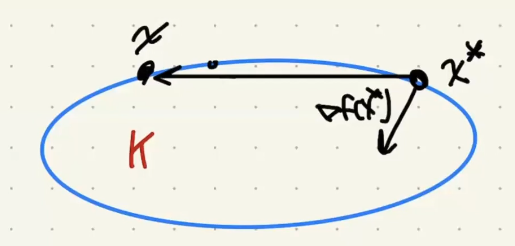
\includegraphics[scale=0.5]{convex_optimality}


\subsection{Derivative of Bregman divergence}

\begin{lemma}
Differentiating Bregman divergence by the first argument gives:
\begin{equation*}
\nabla_x B_\R (x,y) = \nabla \R(x) - \nabla \R(y)
\end{equation*}

\end{lemma}

\subsection{Three point inequality}

\begin{lemma}
The following inequality holds:
\begin{equation*}
B_\R (x,y) + B_\R (y,z) \leq B_\R (x,z) + \pth{\nabla \R(z) - \nabla \R(y)}^T \pth{x-y}
\end{equation*}

\end{lemma}


\section{Online Mirror Descent}

\subsection{Motivation}

There are two meta-algorithms (templates) for online learning that can have sublinear regret bounds. The algorithms that we've seen earlier (Hedge, OGD) can be obtained as private cases of these templates. These two meta-algorithms are:
\begin{itemize}
\item Online Mirror Descent (OMD)
\item Follow the Regularized Leader (FTRL)
\end{itemize}



In the following we look into the OMD meta-algorithm.
We start by looking at an imaginary game with different setting than the regular OCO protocol: now the loss function at each round is known to the player before he makes the decision.
For every $t \in \brk{T} $:
\begin{itemize}
\item The adversary reveals the loss function $ f_t(\cdot) $.
\item The player picks $ x_t \in \Kset $ and incurs loss $ f_t(x_t) $.
\end{itemize}

This setting is much easier than OCO. One possible algorithm in this setting is Best Response:
\begin{equation*}
x_t = \argmin_{x \in \Kset} f_t(x)
\end{equation*} 

\begin{theorem}
Best Response ensures $ \regret_T \leq 0 $.
\end{theorem}

\begin{proof}
By definition
\begin{equation*}
\begin{aligned}
f_t(x_t) & \leq f_t(x), \quad \forall x \in \Kset
\\
\regret_T & = \min_{x \in \Kset} \sum_{t=1}^{T} \pth{f_t(x_t) - f_t(x)} \leq 0
\end{aligned}
\end{equation*}
\end{proof}

Remark: Best Response doesn't require convexity of the loss functions.


\subsection{The algorithm}

We now introduce an algorithm that is inspired by Best Response, but works in the standard OCO setting. Reminder, the OCO protocol is:
For every $t \in \brk{T} $:
\begin{itemize}
\item The player picks $ x_t \in \Kset $.
\item The adversary reveals the loss function $ f_t(\cdot) $.
\item The player incurs loss $ f_t(x_t) $ and receives $ f_t(\cdot) $ as feedback.
\end{itemize}

Let's assume that we have a function (called regularization function) $ \R : \Kset \to \reals $, such that \R{} is \strongcvx{1} \wrt a norm $\norm{\cdot}$.

\begin{algorithm}[H]
\SetKwInput{KwParam}{Parameters}
\SetAlgoLined
\KwParam{ $ \R : \Kset \to \reals $ , $ \eta > 0 $ }
%\KwResult{Write here the result }
$ x_1 = \argmin_{x \in \Kset} \R(x) $
\;
 \For{$t \in \brk{T}$}{
  $ x_{t+1} = \argmin_{x \in \Kset} \pth{ f_t(x) + \frac{1}{\eta} B_\R(x, x_t) } $\;
 }
 \caption{Online Mirror Descent}
\end{algorithm}

Unlike Best Response, this algorithm uses the last observed loss function and not the next one. It uses proximity to the last point to ensure stability of the solution and incorporate information from earlier rounds.

Remarks on linearizing the loss function:
\begin{itemize}
\item If losses are linear the rule becomes $ x_{t+1} = \argmin_{x \in \Kset} \pth{ g_t^T x + \frac{1}{\eta} B_\R(x, x_t) } $.

\item If losses are general convex functions, we can linearize them:

$ g_t = \nabla f_t(x) $; \quad
$ x_{t+1} = \argmin_{x \in \Kset} \pth{ g_t^T x + \frac{1}{\eta} B_\R(x, x_t) } $.

\item Such linearization simplifies the optimization problem.

\item This is a pessimistic approximation of the loss:

$ \forall x: \; f_t(x_t) - f_t(x) \leq \tilde{f}_t(x_t) - \tilde{f}_t(x_t) = \nabla f_t(x_t)^T (x_t - x)$

\item The original loss or another approximation of it may be used instead.

\end{itemize}

Design choices in the OMD algorithm:
\begin{itemize}
\item Regularization function \R{} and the corresponding $ B_\R$.
\item Approximation of the losses.
\item Learning rate $\eta$.
\end{itemize}


\subsection{Regret bound}

We will denote:

\begin{equation*}
D \triangleq \sqrt{ \max_{x} B_\R \pth{ x, \argmin_{y \in \Kset}{\R(y)}}}
\end{equation*}

\begin{equation*}
G \triangleq \mycases{\max_{t \in \brk{T}} \norm{g_t}_* }{\text{linear loss}}{\max_{t \in \brk{T}, x \in \Kset} \norm{ \nabla f_t(x) }_* }{\text{general convex loss}}
\end{equation*}

\begin{theorem}[OMD regret bound]
Setting $ \eta = \frac{D}{G \sqrt{T}} $ guarantees $ \regret_T \leq G D \sqrt{T}$.
\end{theorem}

Note that such $G$ and $D$ may be better than what we've previously had for Hedge and OGD.


\subsection{Private cases}

\subsubsection{OGD}

We will set $ \R(x) = \frac{1}{2} \norm{x}_2^2 $, and use linearized loss.

Then OMD update rule becomes:
\begin{equation*}
\begin{aligned}
x_{t+1}
&= \argmin_{x \in \Kset} \pth{ g_t^T x + \frac{1}{2 \eta} \norm{x - x_t}_2^2 }
\\&= \argmin_{x \in \Kset} \pth{ \frac{1}{2 \eta} \norm{x - x_t + \eta g_t}_2^2 + \text{const} }
\\&= \argmin_{x \in \Kset} \pth{ \norm{x - (x_t - \eta g_t)}_2 }
\\&= \Pi_\Kset^{\norm{\cdot}_2} (x_t - \eta g_t)
\end{aligned}
\end{equation*}

Therefore the update rule in this case is same as OGD.


\subsubsection{Hedge}

We look at the experts setting.

The player decisions lie in the simplex: $ p \in \Kset = \simplex = \braces{ p \in \reals^N, \sum_{i=1}^{N} p(i) = 1, \forall i: p(i) \geq 0 } $.

The loss is a combination of per-expert losses: $ f_t{p} = \L_t^T p $, $ \L_t = \pth{ \L_t(1), \L_t(2), \dots , \L_t(N)} $, $ \L_t(i) \in \brk{0, 1}$

We will use negative entropy as regularization: $ \R(x) = \sum_{i=1}^{N} p(i) \log p(i) $.

Then OMD update rule becomes:
\begin{equation*}
\begin{aligned}
p_{t+1}
&= \argmin_{p \in \simplex} \pth{ \L_t^T p + \frac{1}{\eta} \sum_{i=1}^{N} p(i) \log \frac{p(i)}{p_t(i)} }
\end{aligned}
\end{equation*}

We will solve it ignoring the inequality constraints of \simplex{}, they will be satisfied anyway.
The problem becomes
\begin{equation*}
\argmin_{\sum_{i=1}^{N} p(i) = 1} \pth{ \L_t^T p + \frac{1}{\eta} \sum_{i=1}^{N} p(i) \log \frac{p(i)}{p_t(i)} }
\end{equation*}

Its Lagrangian is:
\begin{equation*}
L(p, \lambda) = \L_t^T p + \frac{1}{\eta} \sum_{i=1}^{N} p(i) \log \frac{p(i)}{p_t(i)} + \lambda \pth{ \sum_{i=1}^{N} p(i) - 1 }
\end{equation*}

\begin{equation*}
\frac{\partial L(p, \lambda) }{\partial p(i)} = \L_t(i) + \frac{1}{\eta} \pth{ \log \frac{p(i)}{p_t(i)} + 1} + \lambda = 0
\end{equation*}

\begin{equation*}
\begin{aligned}
\log \frac{p(i)}{p_t(i)} &= -\eta \L_t(i) - \eta (1 + \lambda)
\\
p(i) &= C p_t(i) e^{-\eta \L_t(i)}, & C = e^{-\eta (1+\lambda)} 
\end{aligned}
\end{equation*}

We need to set $\lambda$ to satisfy the constraints, which is equivalent to setting $C$ to a positive number that satisfies the sum constraint; the non-negativeness constraint is satisfied because $C$, $p_t(i)$ and $e^{-\eta \L_t(i)}$ are all non-negative.

We can also write the decision rule as:
\begin{equation*}
p(i) \propto p_t(i) e^{-\eta \L_t(i)}
\end{equation*}

And if we apply it recursively we get:
\begin{equation*}
\begin{aligned}
p(i) &\propto p_t(i) e^{-\eta \L_t(i)}
\\
&\propto p_{t-1}(i) e^{-\eta \pth{ \L_{t-1}(i) + \L_t(i) }}
\\
&\propto \dots
\\
&\propto p_{1}(i) e^{-\eta \L_{1:t}(i)}
\end{aligned}
\end{equation*}

Recall that $p_1$ must minimize $\R(p)$, which in this case means $ p_1(i) = \frac{1}{N} \quad \forall i $. And this gives us the decision rule that we had in the Hedge algorithm: $ p_{t+1}(i) \propto e^{-\eta \L_{1:t}(i)} $.



\subsection{Proof of regret bound}



%\begin{definition}
%A definition. hypothesis class $\H$.
%\end{definition}
%
%\begin{lemma}
%A lemma.
%\end{lemma}
%
%\begin{theorem}
%A theorem.
%\end{theorem}
%
%\begin{example}
%An example.
%\end{example}

\section{Notation }

We use the following mathematical notation in this writeup:
\begin{itemize}
\item
$d$-dimensional  Euclidean space is denoted $\reals^d$. 
\item
Vectors are denoted by boldface lower-case letters such as $\x \in \reals^d$.  Coordinates of vectors are denoted by regular brackets $\x(i)$ 
\item
Matrices are denoted by boldface upper-case letters such as $\mathbf{X}  \in \reals^{m \times n}$.  Their coordinates by $\mathbf{X}(i,j)$. 
\item
Functions are denoted by lower case letters $f: \reals^d \mapsto \reals$. 

\item 
The $k$-th differential of function $f$ is denoted by $\nabla^k f \in \reals^{d^k}$.  The gradient is denoted without the superscript, as $\nabla f$. 

\item
We use the mathbb macro for sets, such as $\K \subseteq \reals^d$.  

\end{itemize}



%%%%%%%%%%%%%%%%%%%%%%%%%%%%%%%%%%%%%%%%%%%%%%%%%%%%%%%%%%%%%%%%

\end{document}